\documentclass[a4paper, 11pt]{article}
\usepackage{geometry}
\geometry{letterpaper, margin=1in}
\usepackage{amsmath}
\usepackage{amssymb}  
\usepackage{amsthm}
\usepackage{ulem} 
\usepackage{graphicx}
\usepackage{hyperref} 
\begin{document}
\noindent
\large\textbf{HW 9} \hfill \textbf{John Waczak} \\
\normalsize PH 481 \hfill  Date: \today \\
Dr. McIntyre \\

 
\section*{8.38}
\textit{Draw a quartz Wollaston prism, showing all pertinent rays and
	their polarization states.} \\ 

	\begin{figure}[!hbt]
		\centering
		\includegraphics*[width=0.5\columnwidth]{wollastonPrism}
		\caption{\url{https://en.wikipedia.org/wiki/Wollaston_prism}}
	\end{figure}
This figure shows how the Wollaston prism is created from two calcite prisms. The optical axes for each half  are perpendicular to each other. Here blue direction begins as the ordinary axis and the green is the extraordinary. In the second medium, the two axes separate and flip so that the blue axis is extraordinary and the green is ordinary. The beam splitting occurs because the extraordinary beam travels faster in the second prism than the ordinary since $n_e < n_o$. From the vertical view this is: 
	\begin{figure}[!hbt]
		\centering
		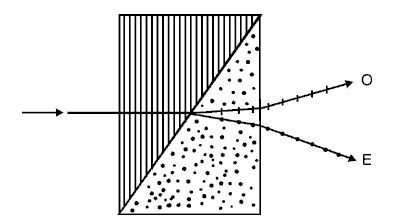
\includegraphics[width = 0.5\columnwidth]{wollastonTop}
		\caption{\url{https://pe2bz.philpem.me.uk/Lights/-\%20Laser/Info-902-LaserCourse/c06-07/mod06_07.htm}} 
	\end{figure}
	
\section*{8.55}
\textit{Take two ideal Polaroids (the first with its axis vertical and the
	second, horizontal) and insert between them a stack of 10 half-wave
	plates, the first with its fast axis rotated $\pi/40$ rad from the vertical, and
	each subsequent one rotated $\pi/40$ rad from the previous one. Deter-
	mine the ratio of the emerging to incident irradiance, showing your
	logic clearly.}\\

First, recall the law of Malus which states that the intensity of linearly polarized light that pases through a linear polarizer as a function of the angular difference is 
	\begin{equation*}
		I(\theta) = I_0\cos^2\theta
	\end{equation*}
If we assume that the incoming light is natural i.e. randomly polarized (other polarizations would require another application of Malus's law) than after passing through the first polarizer we would have that the intensity is given by $I_0 = I/2$ where $I$ is the incident polarization. Then all we need to do is figure out how the wave plates change the polarization of the beam while it is in between the polarizers. Once we know it's final phase we can apply Malus's law to find the exiting intensity. Since $n_e \neq n_o$ the waves travel at different speeds. A half-wave plate introduces $\pi$ difference between the two components. If the plate is tilted at an angle $\phi$ then the effect is to tilt the polarization of a linearly polarized light by $2\phi$. Thus we have the total tilt of the initial polarization $\Phi$ is:
	\begin{align*}
		\Phi &= 2\phi*10 \\ 
			& 20\frac{\pi}{40} \\
			& = \frac{\pi}{2}
	\end{align*}
Thus what was vertically polarized light is now horizontal and so $\theta = 0$. This means that $I_{exit} = \frac{I}{2}$ and so the ratio is given by: 
	\begin{equation*}
		\frac{I_{exit}}{I_{inc}} = \frac{I/2}{I} = \frac{1}{2}
	\end{equation*}
	
\section*{8.71}
\textit{The specific rotatory power for sucrose dissolved in water at
	20°C ($\lambda_0$ = 589.3 nm) is + 66.45° per 10 cm of path traversed through
	a solution containing 1 g of active substance (sugar) per $cm^3$ of solution. A vertical P-state (sodium light) enters at one end of a 1-m tube
	containing 1000 $cm^3$ of solution, of which 10 g is sucrose. At what
	orientation will the P-state emerge?}\\

Recall from lab that the equation for the specific rotatory power is given by: 
	\begin{equation*}
		[\alpha]_\lambda^T = \frac{\beta}{dc}
	\end{equation*}
	
where $\beta$ is the angle of rotation of the plane of the light beam, $d$ is the distance traveled in the medium, and $c$ is the concentration in $[g/cm^3]$. Let's use the given information to calculate $\alpha$. 
	\begin{align*}
		\alpha = \frac{66.45}{1\cdot 10} = 6.645
	\end{align*}

Now all we need to do is find the new concentration and apply the specific rotatory 
	\begin{align*}
		c = \frac{m}{V} = \frac{10\text{ g}}{1000 \text{}cm^3} = 0.01\text{ g/cm3}
	\end{align*}
and so we have that:
	\begin{align*}
		\beta &= \alpha d c \\ 
			&= 6.645\text{ deg cm2/g}\cdot 100\text{ cm} \cdot 0.01 \text{g/cm3} \\
			&= 6.645^{\circ}
	\end{align*} 
Since the light was prepared in the $\mathbb{P}$ state we have that the final angle will be $6.645^{\circ}$ from the vertical or $96.645^{\circ}$ from the horizontal.
 
\section*{13.45}
\textit{A diffraction grating having a mere 50 grooves per cm is the
	object in the optical computer shown in Fig. 13.41(I think this is a typo in the book). If it is coherently illuminated by plane waves of green light (543.5 nm) from a He-Ne laser and each lens has a 100-cm focal length, what will be the spacing of the diffraction spots on the transform plane?} \\

If there are 50 grooves per centimeter then we can define the "slit width" i.e. the grating spacing to be $a=1/50$ cm $= 1/5000$ m. If the focal length of the lens is $f = 100$ cm $=1$ m then we have that:
	\begin{equation*}
		a\sin\theta = m\lambda
	\end{equation*}
Now using the small angle approximation we have $\sin\theta \approx \tan\theta = y/f$ Since we are at the focal length. Therefore taking $m=1$ gives: 
	\begin{align*}
		a\frac{y}{f} &= \lambda \\ 
		y &= \frac{\lambda f}{a} \\ 
			&= 543.5e-9\cdot 1.00\cdot 5000 \\ 
			&= 0.00272 m = 2.72 mm 
	\end{align*}

\section*{13.46} 
\textit{Imagine that you have a cosine grating (i.e., a transparency
	whose amplitude transmission profile is cosinusoidal varying between
	0 and 1) with a spatial period of 0.01 mm. The grating is illuminated
	by quasimonochromatic plane waves of l = 500 nm, and the setup is
	the same as that of Fig. 13.36, where the focal lengths of the transform
	and imaging lenses are 2.0 m and 1.0 m, respectively.}
\subsection*{a}
\textit{Discuss the resulting pattern and design a filter that will pass only
	the first-order terms. Describe it in detail.}\\
	
	Our lens is performing a Fourier transform on the cosine grating. Thus the pattern will be a pair of $\delta$ functions centered at $\pm d$ where d is the spatial frequency of the cosine. In order to pass only first oder terms we need to create a filter that will block out only these delta functions i.e. two opaque dots at $\pm d$. For the specific wavelength given we can calculate this distance using the small angle approximation. 
		\begin{align*}
			a\frac{d}{f} \approx a\sin\theta &= m\lambda \\ 
			\Rightarrow d &= \frac{f\lambda}{a}\text{ m=1} \\ 
				&= 2\cdot 500e-9\cdot 100 \\
				&= 0.1 \text{ mm} 
		\end{align*} 
	Thus we need opaque dots at $\pm 0.1$ mm from the center. 
\subsection*{b}
\textit{What will the image look like on $\Sigma_i$ with that filter in place?}\\
	If we want to only allow the first order terms we can make a black screen with two transparent dots at $\pm d$. This would allow only light from those to pass (removing the DC zero sptial frequency term) and result in a clear cosine intensity in the viewing plane (i.e. you get the grating pattern back). The only caveat is that we measure intensities so this would really be a cosine squared and thus we would lose some phase information. 

\subsection*{c}
\textit{How might you pass only the DC term, and what would the image
	look like then?}\\
	
	To pass only the DC term we could to the reverse of part (b) and instead black out everything except for the central m=0 DC spot. This would "remove" the cosine grating and result in a uniform intensity in the viewing plane. This essentially gives us what the light looked like before it entered the grating. 
\end{document}



















